\documentclass[12pt, letterpaper, oneside, openany draft, spanish]{book} % book for the frontmatter and mainmatter
\title{Pasantia}
\author{José Ricardo Pascarella Quijada} 
\date{\today}

\usepackage[spanish]{babel} %Lenguaje Español
\usepackage[utf8]{inputenc} %Paquete para escribir acentos y otros símbolos directamente

% for development %
% \includeonly{capitulos/1, Introduccion}

% \usepackage{syntonly}
% \syntaxonly

% Tamanos de las fuentes
% 12pt option
% \tiny         	6pt
% \scriptsize     8pt
% \footnotesize   10pt
% \small         	11pt
% \normalsize     12pt
% \large         	14pt
% \Large         	17pt
% \LARGE         	20pt
% \huge         	25pt	
% \Huge         	25pt


\pagestyle{myheadings} % para solo tener los numeros en el tope

\linespread{1.3} % Entre lineas de 1,5. Lo se, es raro

\setlength{\parskip}{10pt} % Doble espacio entre parrafos !!!!!!!!!!!!! Medir esto con un word

\usepackage[left=3cm,top=2cm,right=2cm,bottom=2cm,bindingoffset=0.5cm]{geometry} 
\usepackage{xcolor,graphicx}

% Capitulos en tamano 14 negrita, centrados con el nombre abajo y en mayusculas
\usepackage{titlesec}
\titleformat{\chapter}[display]   
{\normalfont\large\bfseries\centering}{\MakeUppercase{\chaptertitlename\ \thechapter}}{-10pt}{\bfseries\normalsize\MakeUppercase}
\titlespacing*{\chapter}{0pt}{0cm}{0cm}

% Secciones y subsecciones en tamano 12 y negrita
\titleformat*{\section}{\normalsize\bfseries}

\titleformat*{\subsection}{\normalsize\bfseries}

\begin{document}

\frontmatter % Numeracion Romana

\begin{titlepage}
\begin{center}

\begin{figure}[h]
\begin{center}

\includegraphics{Logos/logoUSB.png}
\end{center}
\end{figure}

\textsc{UNIVERSIDAD SIMÓN BOLÍVAR}\\
\textsc{DECANATO DE ESTUDIOS PROFESIONALES}\\
\textsc{COORDINACIÓN DE INGENIRÍA DE LA COMPUTACIÓN}\\[8em]

\textsc{\Large \textbf{EXTENSIÓN DE UN SISTEMA DE MANEJO DE APRENDIZAJE CON UN MÓDULO DE ENCUENTROS PRESENCIALES}}\\[4em]

\textsc{ \textbf{Por:} }\\
José Ricardo Pascarella Quijada\\[4em]

\textsc{ \textbf{INFORME DE PASANTÍA} }\\
Presentado ante la Ilustre Universidad Simón Bolívar\\
como requisito parcial para optar al título de \\
Ingeniero en Computación

\vspace*{\fill}

\textsc{ \textbf{Sartenejas, Septiembre de 2017} }
\end{center}
\end{titlepage}

\thispagestyle{empty} % No number in the tittle page
\begin{center}

\begin{figure}[h]
\begin{center}

\includegraphics{Logos/logoUSB.png}
\end{center}
\end{figure}

\textsc{UNIVERSIDAD SIMÓN BOLÍVAR}\\
\textsc{DECANATO DE ESTUDIOS PROFESIONALES}\\
\textsc{COORDINACIÓN DE INGENIRÍA DE LA COMPUTACIÓN}\\[8em]

\textsc{\Large \textbf{EXTENSIÓN DE UN SISTEMA DE MANEJO DE APRENDIZAJE CON UN MÓDULO DE ENCUENTROS PRESENCIALES}}\\[4em]

\textsc{ \textbf{Por:} }\\
\textsc{José Ricardo Pascarella Quijada}

\textsc{ \textbf{Realizado con la asesoría de:} }\\
\textsc{Prof. Federico Flaviani }\\
\textsc{Ing. Christian Ament}\\[4em]

\textsc{ \textbf{INFORME DE PASANTÍA} }\\
\textsc{Presentado ante la Ilustre Universidad Simón Bolívar}\\
\textsc{como requisito parcial para optar al título de }\\
\textsc{Ingeniero en Computación}

\vspace*{\fill}

\textsc{ \textbf{Sartenejas, Septiembre de 2017} }
\end{center}


% Para meter los graficos del acta escaneada
\mbox{}
\thispagestyle{empty}
\newpage

\mbox{}
\thispagestyle{empty}
\newpage

\begin{center}
	
	\begin{figure}[h]
		\begin{center}
		
\includegraphics[width=0.1\textwidth]{logos/logoUSB.png}
		\end{center}
	\end{figure}

	\textsc{UNIVERSIDAD SIMÓN BOLÍVAR}\\[0.1pt]
	\textsc{DECANATO DE ESTUDIOS PROFESIONALES}\\
	\textsc{COORDINACIÓN DE INGENIERÍA DE LA COMPUTACIÓN}

	\textsc{\textbf{EXTENSIÓN DE UN SISTEMA DE GESTIÓN DE APRENDIZAJE CON UN MÓDULO DE ENCUENTROS PRESENCIALES}}

	Realizado por: José Ricardo Pascarella Quijada\\
	Con la asesoría de:	Prof. Federico Flaviani e Ing. Christian Ament

	\textsc{\textbf{RESUMEN}}

\end{center}

Este documento presenta detalladamente el proceso de desarrollo de una extensión para un \gls{SGA} que permite el soporte de encuentros presenciales o seminarios entre estudiantes e instructores. 

El módulo apoya a tres tipos de usuarios en la gestión de los encuentros. Los administradores, que crean los cursos y asignan los instructores. Los instructores que pueden administrar la asistencia y calificación; por último, los estudiantes que seleccionan cursos a los que asistir.

Para la realización de este módulo se usó la metodología de desarrollo de \emph{software} ágil e iterativo por fases \emph{scrum}. Para el desarrollo se utilizó el conjunto de soluciones informáticas \gls{WAMP}, que consiste en Windows como plataforma de sistema operativo, Apache para el servicio web, \gls{SQL} Server con gestor de bases de datos y el lenguaje multipropósito \gls{PHP}.

Se logró mediante este proyecto que el SGA base de la compañía contenga la nueva funcionalidad, que permite ser extendida y personalizada dependiendo de las necesidades de distintos clientes. Además, el módulo se implantó con éxito en la arquitectura de un cliente que previamente poseía el servicio de \gls{SGA}.

\textbf{Palabras clave}: \gls{SGA}, \gls{PHP}, desarrollo, seminario.






\chapter*{Dedicatoria}

A mi madre que me ha dedicado su vida

A mi padre que siempre me apoya y nunca deja de aconsejarme

A mi tía Evelin que me tomó en serio desde los 8 años, mucho antes de que yo lo hiciera 

Los amo. 

\chapter*{Agradecimientos}

A mis padres y mi tía Evelin, por ser siempre un impulso y un apoyo que me ha permitido llegar a lugares a los que nunca me hubiese imaginado, gracias a ustedes puedo decir que nunca me ha faltado nada, sobre todo amor.

Al resto de la familia por propiciar el mejor ambiente para mi desarrollo, en ustedes constantemente encuentro ejemplos a seguir, consejos, cariño y una inmesa responsabilidad de recordar de donde vengo con orgullo compartir los valores que de ustedes y con ustedes aprendí. 

A Clara Cangiano, te separo aqui de la familia, pero solo para que sepas que a ella perteneces. Gracias por compartir toda tu vida conmigo, de ti he aprendido mucho. El amor sin una cesta llena haz como que no lo has visto. Siempre mantuviste la cesta llena. No creas que olvidaré la promesa que te hice.

A mis amigos mas cercanos, cada uno con un aporte muy especial: Guillermo Hernández, con el que siempre fue bueno competir, pero al mismo tiempo me recordó ser humilde, no te quedes atras. Luis Colorado, una de esas personas que a veces no te crees que existen, su entrega y positividad es única. Rafael Delgado, siempre estas allí viejo, nos veremos pronto. Mailyn Guevara por lo fácil que es compartir todo contigo y Fabiana Abdallah, gracias a tí valoro la sinceridad y entiendo que se puede conseguir.

A la gente del Laboratorio Docente de Aulas Computarizadas (MAC). No solo por ser mi casa en Caracas, si no por hacer de esa casa un hogar. Compartir con ustedes cada día fue una experiencia única de aprendizaje y superación sobre la computación y la vida. La mejor decisión que he tomado es hacer esa admisión.

A todas las demás personas que hacen vida en la Universidad Simón Bolívar, junto y gracias a ustedes no solo me formé como ingeniero, dadas las circunstancias, aprendí que hay que luchar, que la vida no es fácil, junto a ustedes estuve luchando en todos los frentes codo a codo y el que se roza con diamantes de alguna forma se pule.

Luis Colorado y Andres Navarro, gracias por hacer los últimos pasos no solo amenos, sino posibles, que viva el tridente.

% \tableofcontents % Indice

% \listoftables

\mainmatter % Comienzo de numeracion arabica

\chapter*{Introducción}
\thispagestyle{empty} % Quitar el número
\addcontentsline{toc}{chapter}{Introducción} \markboth{INTRODUCCIÓN}{}
El presente documento describe el proceso de desarrollo del módulo de encuentros presenciales para un SAG (Sistema de Gestión de Aprendizaje) para Fischer Knoblauch \& Co (FKC) como proyecto de pasantías realizado por su autor.

\section*{Antecedentes}
\addcontentsline{toc}{section}{Antecedentes}
El SGA básico de FKC es un producto que soporta las funciones basicas de cualquier sistema de gestión aprendizaje simple. Como lo son: manejo de usuarios y contenidos; segimiento del proceso de aprendizaje, evaluaciones y herramientas de comunicación como foros y mensajes privados. Este sistema es personalizado e instalado generalmente en la infraestructura del cliente según sus necesidades.

\section*{Justificación e importancia}
\addcontentsline{toc}{section}{Justificación e importancia}
Entre las funciones convencionales de los SGA actuales se encuentra el manejo de encuentros presenciales, funcionalidad considerada como necesaria por actuales y potenciales clientes. Siendo estos encuentros de importancia crítica para el flujo del conocimiento de mediana a alta complejidad que no puede ser expresado facilmente por medio de cursos en linea. Por lo tanto, es de interés para la compañia poseer esta funcionalidad en su sistema.


\section*{Planteamiento del problema}
\addcontentsline{toc}{section}{Planteamiento del problema}
Se identificó la necesidad de extender el sistema de FKC con un módulo que le permita a sus clientes gestionar encuentros presenciales entre instructores y estudiantes. Al mismo tiempo este módulo debía adaptarse a la estructura de cursos y grupos previamente existente en el sistema trantando de incluir la menor complejidad posible para su futura extensión y personalización.

Para lograr esto, es necesario un profundo entendimiento del producto, con el fin de desarrollar un módulo que mantenga el mismo estilo tanto en la programacion, como en el funcionamiento y la interfaz. 


\section*{Objetivos}
\addcontentsline{toc}{section}{Objetivos}
A continuación, se exponen los objetivos generales y específicos que se busca alcanzar en este desarrollo con la finalidad de contextualizar al lector respecto al informe de este proyecto de pasantía.

\subsection*{Objetivo general}
\addcontentsline{toc}{subsection}{Objetivo general}
El objetivo general de este proyecto es desarrollar un módulo que permita extender el sistema de gestión de aprendizaje con un módulo que lo acerque a contener las funciones convencionales de los sistemas en la actualidad y que al mismo tiempo posea la flexibilidad de ser personalizado para las distintas necesidades de los clientes o hasta no ser incluido de no ser necesario.

\subsection*{Objetivos específicos}
\addcontentsline{toc}{subsection}{Objetivos específicos}
Extender la Base de Datos para el soporte del módulo.

Desarrollo de un módulo que permita el manejo de las locaciones donde se imparten los seminarios por parte del administrador.

Integrar el nuevo tipo de curso a las funcionalidades previas de administrador sobre otros tipos de cursos, como estadísticas y asignación a grupos.

Creación de un nuevo tipo de usuario, instructor, que tenga potestad sobre los seminarios.

Integrar el nuevo tipo de cursos en la interfaz del estudiante del sistema.

Integrar el módulo tanto en el sistema base de FKC como en uno de los clientes que poseen un versión personalizada del sistema.










\chapter{Entorno Empresarial}
\thispagestyle{empty} % Quitar el número

En este capítulo se describe el entorno empresarial en el cual tuvo lugar el desarrollo del proyecto de pasantía, la empresa \gls{FKC} filial de Frankfurt.

\section{Fischer, Knoblauch \& Co.}

Es un proveedor de servicios multimedia especializado en el área de aprendizaje electrónico. Está presente en Frankfurt y Munich en Alemania así como en Basel, Suiza. Fundada en 1996 por Guy Fischer y Thomas Knoblauch.

Proveen consultoría en la integración y ampliación del aprendizaje electrónico a compañías de diversos sectores en Alemania y Bélgica. Se encargan de sugerir la elección de tecnologías, concepción del plan de aprendizaje, didácticas y metodología de la enseñanza, producción del contenido audiovisual, hasta la integración de la solución en el ambiente del cliente. 

Si una compañía requiere enseñar una cierta habilidad a sus empleados contacta a un proveedor de servicios de aprendizaje electrónico, \gls{FKC} los ayuda a integrar un plan aprendizaje a su empresa, que se ven materializados en entrenamientos basados en la web. 

\gls{FKC} también posee un Sistema de Gestión de Aprendizaje, la pieza de \emph{software} en la que el pasante trabajó, que es personalizable y permite la organización de estos entrenamientos creados por la empresa.

Además, \gls{FKC} haciendo uso de su departamento gráfico y programadores, también provee servicios de posicionamiento empresarial en la web, mediante la creación de páginas, logos y demás contenido multimedia que la compañía requiera. 

Sus programadores día a día se enfrentan con diversos retos informáticos en distintos lenguajes de programación. Estos pueden ser: migraciones de sistemas de bases de datos, internacionalización de sus aplicaciones que llegan a estar hasta en diez lenguajes distintos, diseño de soluciones multiplataforma y el manejo e instalación de \emph{frameworks} que faciliten la construcción de soluciones multimedia.

\section{Estructura organizacional}

En la figura \ref{fig:estructuraFKC} se muestra la estructura organizacional de \gls{FKC} Frankfurt:

\begin{figure}[h]
\begin{center}
	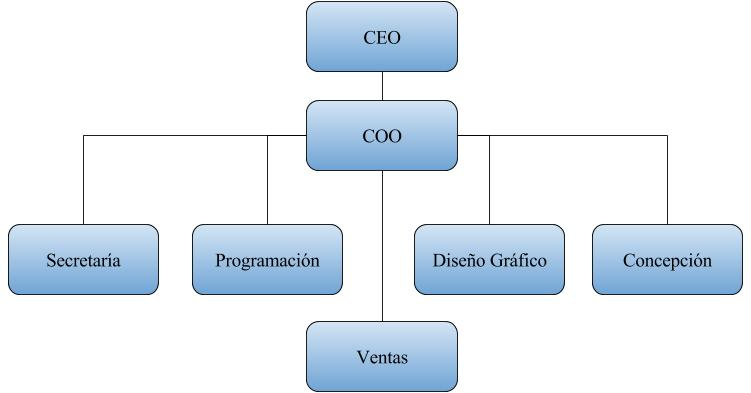
\includegraphics[width=\textwidth]{figuras/estructuraFKC.jpg}
	\caption{Estructura organizacional de \gls{FKC}.} \label{fig:estructuraFKC}
\end{center}
\end{figure}

\gls{FKC} Frankfurt es un equipo multidisciplinario donde es importante la comunicación entre los distintos \emph{stakeholders}. Los creadores de concepto se unen a los diseñadores y los programadores para plasmar fielmente los requerimientos del cliente y obtener como resultado una solución hecha a la medida.

A continuación una descripción breve de los cargos en el organigrama.

Director Ejecutivo es la persona de máxima autoridad, encargada de la gestión y dirección administrativa en la organización.

Director de Operanciones es el responsable del control de las actividades diarias de la corporación y de manejo de las operaciones. Reporta directamente al director ejecutivo.

Secretaría encargada de dar apoyo a los empleados de la empresa en cuanto a la gestión de papeleo y la comunicación de las actividades.

La cuadrilla de programación se encarga de materializar las peticiones que llegan de los demás departamentos mediante soluciones informáticas.

El grupo de diseño gráfico se encarga de generar el material multimedia junto con los integrantes del grupo de concepción y los clientes. 

El departamento de ventas se encarga del \emph{marketing} de los productos ofrecidos por \gls{FKC}.

\section{Cargo ocupado por el pasante} 

El pasante perteneció al grupo de programación que se muestra en la figura \ref{fig:estructuraFKC} donde formó parte de un equipo de 6 programadores.






\end{document}